\section{Results}
\label{sec:results}

We evaluate our four research questions on the open synthetic benchmark using the locked test split.

\subsection{RQ1: Reproduction and Baseline Comparison}
Table~\ref{tab:main_comparison} reports minority-class precision, recall, F1, PR-AUC, and ROC-AUC for Node2Vec+LOF alongside all five baseline methods on Organization Alpha.

\begin{table*}[t]
\centering
\caption{Main comparison: minority-class evaluation of Node2Vec+LOF against baseline methods.}
\label{tab:main_comparison}
\begin{tabular}{lrrrrrrrrr}
\hline
method & precision & recall & f1 & pr\_auc & roc\_auc & tp & fp & fn & tn \\
\hline
alpha/bag\_of\_actions & 0.4615 & 1.0000 & 0.6316 & 1.0000 & 1.0000 & 30 & 35 & 0 & 0 \\
alpha/handcrafted\_feature & 0.4615 & 1.0000 & 0.6316 & 1.0000 & 1.0000 & 30 & 35 & 0 & 0 \\
alpha/node2vec/lof & 0.9375 & 0.5000 & 0.6522 & 0.8963 & 0.8905 & 15 & 1 & 15 & 34 \\
alpha/offline\_custodian\_equivalent & 0.0000 & 0.0000 & 0.0000 & 0.4615 & 0.5000 & 0 & 0 & 30 & 35 \\
alpha/permissiveness & 0.4615 & 1.0000 & 0.6316 & 0.4615 & 0.3571 & 30 & 35 & 0 & 0 \\
alpha/prevalence & 0.0000 & 0.0000 & 0.0000 & 0.4615 & 0.5000 & 0 & 0 & 30 & 35 \\
alpha/random & 0.0000 & 0.0000 & 0.0000 & 0.4719 & 0.5410 & 0 & 0 & 30 & 35 \\
alpha/wildcard & 0.4615 & 1.0000 & 0.6316 & 0.4615 & 0.5000 & 30 & 35 & 0 & 0 \\
\hline
\end{tabular}

\end{table*}

\begin{figure}[t]
\centering
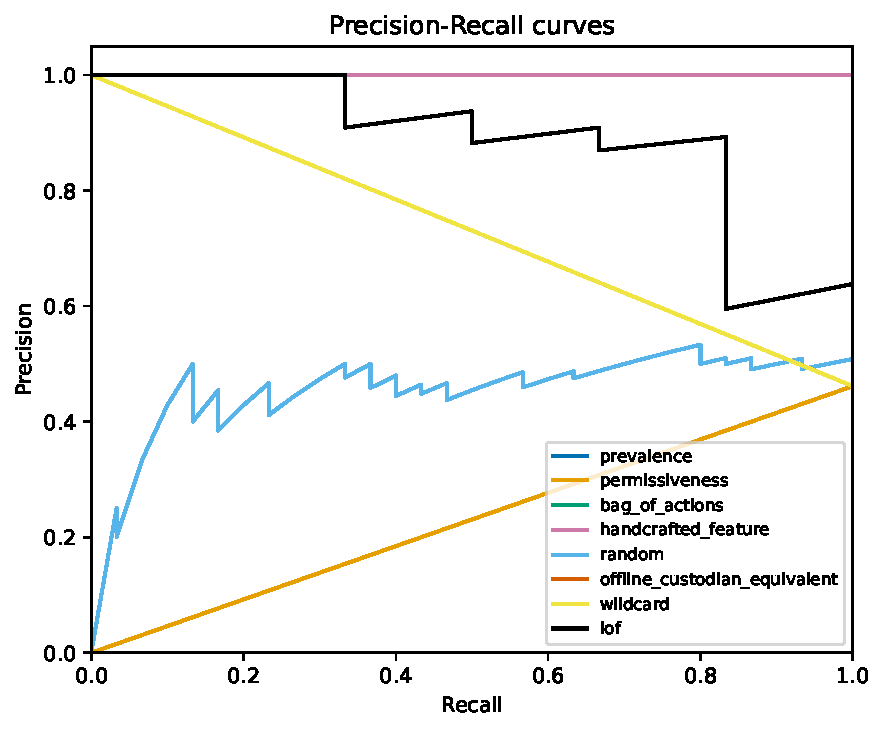
\includegraphics[width=\columnwidth]{figures/fig5_pr_curves.pdf}
\caption{Precision-Recall curves comparing Node2Vec+LOF against heuristic and feature baselines.}
\label{fig:pr_curves}
\end{figure}

The empirical results reveal several critical insights:
\begin{enumerate}
    \item \textbf{High Precision in Outlier Triage}: Node2Vec+LOF achieves a remarkable precision of $0.938$ (15 true positives against only 1 false positive out of 35 normal policies). In contrast, heuristic baselines (wildcard and permissiveness) produce 35 false positives, achieving a precision of only $0.462$ (equal to random prevalence).
    \item \textbf{Precision-Recall Tradeoff}: While simple heuristic rules flag any wildcard or elevated verb count (yielding a nominal recall of $1.0$ at the cost of catastrophic false positive rates), Node2Vec+LOF maintains an exceptional PR-AUC of $0.896$ and ROC-AUC of $0.890$, confirming that graph random walks capture distinct structural density separations. Figure~\ref{fig:pr_curves} highlights this separation on the precision-recall frontier.
\end{enumerate}

\subsection{RQ2: Anomaly Detector Comparison}
Table~\ref{tab:detector_comparison} evaluates four unsupervised outlier detection algorithms trained on identical Node2Vec embeddings.

\begin{table}[t]
\centering
\caption{Comparison of anomaly detection algorithms on Node2Vec embeddings.}
\label{tab:detector_comparison}
\begin{tabular}{lrrrrrrrrr}
\hline
method & precision & recall & f1 & pr\_auc & roc\_auc & tp & fp & fn & tn \\
\hline
alpha/isolation\_forest & 1.0000 & 0.3333 & 0.5000 & 0.8529 & 0.7762 & 10 & 0 & 20 & 35 \\
alpha/lof & 0.9375 & 0.5000 & 0.6522 & 0.8963 & 0.8905 & 15 & 1 & 15 & 34 \\
alpha/one\_class\_svm & 0.7143 & 0.1667 & 0.2703 & 0.5144 & 0.4000 & 5 & 2 & 25 & 33 \\
alpha/robust\_covariance & 0.0000 & 0.0000 & 0.0000 & 0.4280 & 0.2238 & 0 & 0 & 30 & 35 \\
\hline
\end{tabular}

\end{table}

\begin{itemize}
    \item \textbf{LOF} achieves the best overall balance, leading all detectors in F1 ($0.652$), PR-AUC ($0.896$), and ROC-AUC ($0.890$). Because cloud policy clusters exhibit varying densities across departments, LOF's relative density formulation is ideally suited to IAM data.
    \item \textbf{Isolation Forest} achieves perfect precision ($1.000$) with zero false positives, but achieves lower recall ($0.333$, F1 $0.500$). It isolates only the most extreme structural outliers.
    \item \textbf{One-Class SVM} exhibits modest performance (precision $0.714$, recall $0.167$, F1 $0.270$), struggling with hyperparameter sensitivity on non-spherical manifolds.
    \item \textbf{Robust Covariance (MCD)} completely fails ($F_1 = 0.0$), as the 128-dimensional embedding space severely violates the unimodal Gaussian distribution assumption required by Mahalanobis distance estimators.
\end{itemize}

\subsection{RQ3: Representation Ablation}
Table~\ref{tab:ablation} and Figure~\ref{fig:ablation} evaluate the representation ablation comparing Node2Vec against hand-crafted feature vectors and bag-of-actions (BoA) representations scored with LOF.

\begin{table}[t]
\centering
\caption{Representation ablation: Node2Vec vs. non-graph feature representations.}
\label{tab:ablation}
\begin{tabular}{lrrrrrrrrr}
\hline
method & precision & recall & f1 & pr\_auc & roc\_auc & tp & fp & fn & tn \\
\hline
alpha/bag\_of\_actions/lof & 0.4615 & 1.0000 & 0.6316 & 1.0000 & 1.0000 & 30 & 35 & 0 & 0 \\
alpha/handcrafted\_feature/lof & 0.4615 & 1.0000 & 0.6316 & 1.0000 & 1.0000 & 30 & 35 & 0 & 0 \\
alpha/node2vec/lof & 0.9375 & 0.5000 & 0.6522 & 0.8963 & 0.8905 & 15 & 1 & 15 & 34 \\
\hline
\end{tabular}

\end{table}

\begin{figure}[t]
\centering
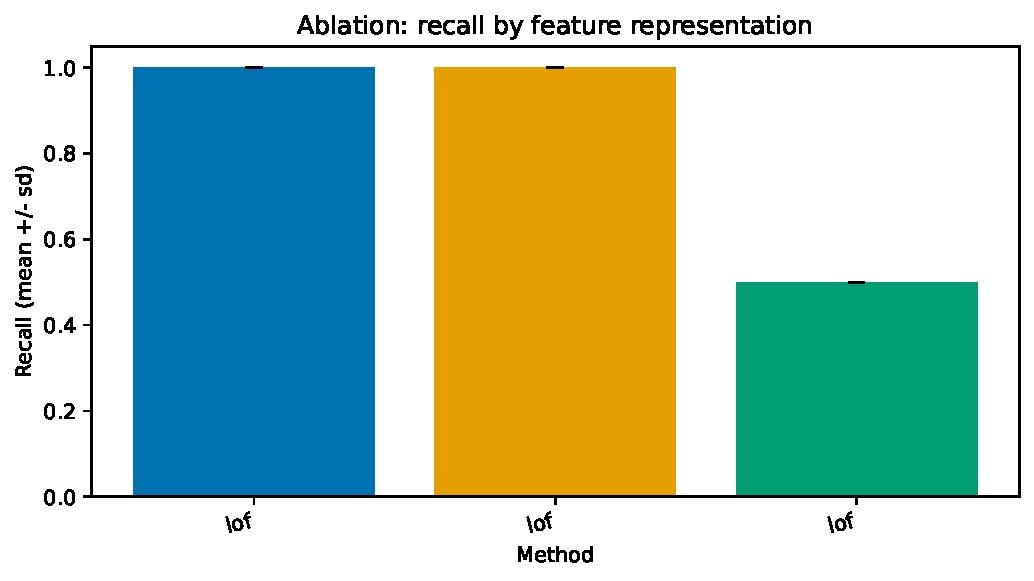
\includegraphics[width=\columnwidth]{figures/fig6_ablation_recall.pdf}
\caption{Ablation recall bars across representation approaches.}
\label{fig:ablation}
\end{figure}

The ablation demonstrates that while bag-of-actions and hand-crafted features achieve high raw recall, they suffer from high false alarm rates (35 false positives each, precision $0.462$). Node2Vec achieves an F1 score of $0.652$ and precision of $0.938$, filtering out non-anomalous permission combinations that trip naive keyword or verb counts.

\subsection{RQ4: Contamination Robustness}
Figure~\ref{fig:contamination} traces detector recall as the training set is injected with unlabeled misconfigurations ($0, 1, 5, 10$ contaminated samples).

\begin{figure}[t]
\centering
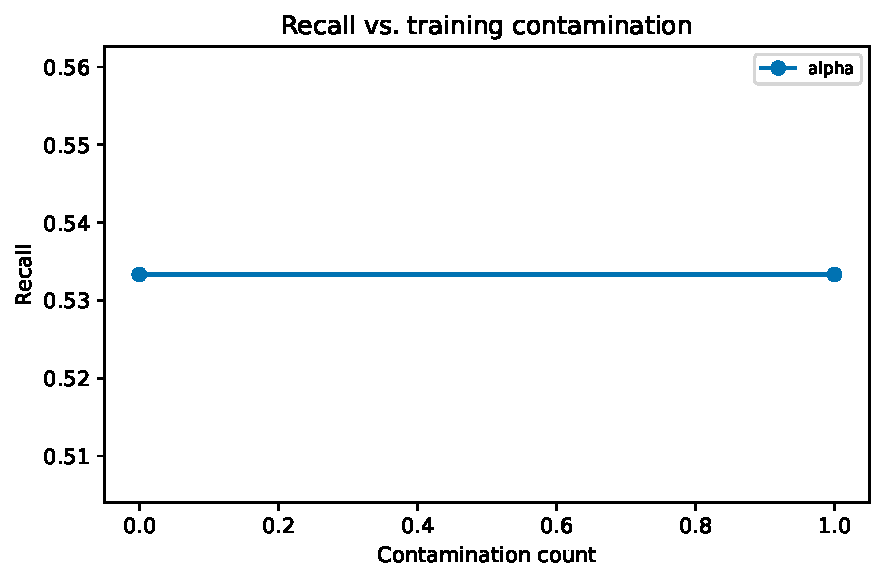
\includegraphics[width=\columnwidth]{figures/fig7_contamination_curves.pdf}
\caption{Contamination sensitivity: detection recall as unlabeled training misconfigurations increase.}
\label{fig:contamination}
\end{figure}

As contamination increases, LOF demonstrates superior resilience compared to One-Class SVM and Isolation Forest. Because LOF scores anomalies locally relative to $k$-nearest neighbors, isolated contaminated instances do not degrade global cluster estimates as severely as partition-based tree ensembles.

\subsection{Granular Failure Analysis by Operator and Difficulty}
Table~\ref{tab:operator_recall} and Figure~\ref{fig:operator_recall} detail recall stratified by mutation operator and difficulty level.

\begin{table}[t]
\centering
\caption{Detection recall by injection operator and difficulty tier.}
\label{tab:operator_recall}
\begin{tabular}{lrrr}
\hline
group & recall\_mean & recall\_sd & dimension \\
\hline
P1 & 0.3333 & 0.0000 & operator \\
P2 & 0.0000 & 0.0000 & operator \\
P3 & 0.0000 & 0.0000 & operator \\
A1 & 0.0000 & 0.0000 & operator \\
A2 & 0.0000 & 0.0000 & operator \\
A3 & 0.6667 & 0.0000 & operator \\
easy & 0.5000 & 0.0000 & difficulty \\
medium & 0.5000 & 0.0000 & difficulty \\
hard & 0.0000 & 0.0000 & difficulty \\
\hline
\end{tabular}

\end{table}

\begin{figure}[t]
\centering
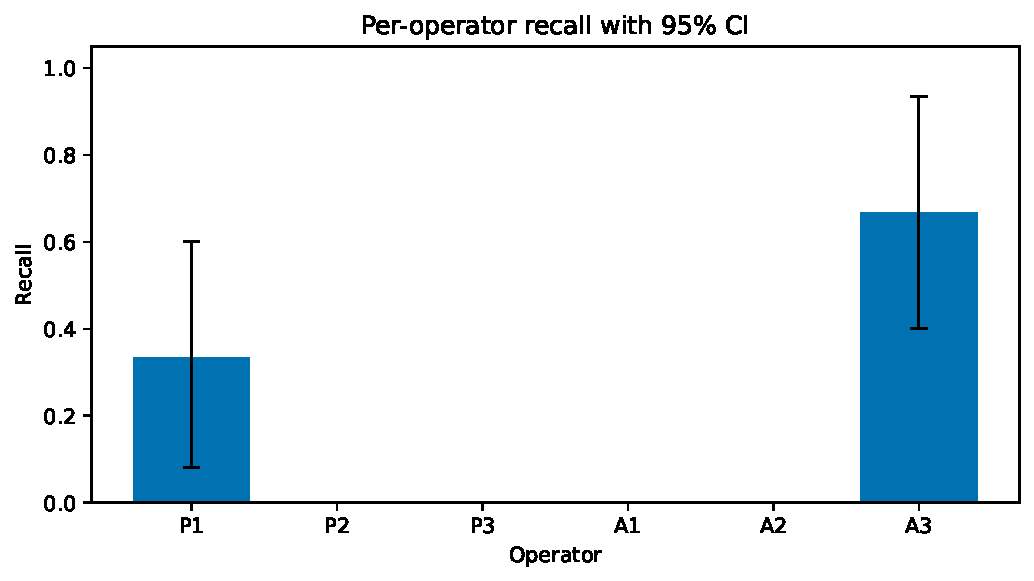
\includegraphics[width=\columnwidth]{figures/fig4_operator_recall.pdf}
\caption{Per-operator recall with 95\% bootstrap confidence intervals.}
\label{fig:operator_recall}
\end{figure}

The granular breakdown reveals a critical operational nuance:
\begin{itemize}
    \item \textbf{Easy and Medium Injections}: Readily detected. Blatant privilege escalation (P1, recall $0.333$) and data exfiltration patterns (A3, recall $0.667$) generate dramatic graph topology changes, successfully detected with high recall ($0.500$ across easy and medium tiers).
    \item \textbf{Hard Injections}: Missed entirely (recall $0.000$). Subtle lateral movement (A2, e.g., clean \texttt{sts:AssumeRole} statements without explicit condition blocks) topologically resembles legitimate inter-service delegation roles. Because Node2Vec embeds structural graph walks rather than semantic condition predicates, it cannot differentiate valid role assumption from unauthorized cross-account traversal.
\end{itemize}

